% SSC 2026 Workshop - Segment C: Foundations
% Kathryn Morrison  (10:45 - 11:25)
% Theme and structure recycled from Andy Wilson's Module 1 deck.

\documentclass[aspectratio=169]{beamer}

% Theme and packages
\usetheme{metropolis}
\usepackage[utf8]{inputenc}
\usepackage{amsmath, amssymb, mathtools, bm}
\usepackage{graphicx}
\usepackage{booktabs}
\usepackage{lmodern}
\usefonttheme{professionalfonts}
\usepackage{microtype}
\usepackage{xcolor}
\usepackage{hyperref}
\usepackage[absolute,overlay]{textpos}
\usepackage{tikz}
\usetikzlibrary{positioning,arrows.meta,shapes.geometric,calc}
\usepackage[numbers]{natbib}

\title[Foundations]{Foundations}
\subtitle{Segment C \textbullet\ Modern Analysis of Real-World Data}
\author{Kathryn Morrison}
\institute{instats SSC 2026 Accreditation Workshop}
\date{}

\definecolor{accent}{HTML}{4A9EFF}
\definecolor{brick}{HTML}{C0392B}
\definecolor{good}{HTML}{27AE60}
\definecolor{inkdark}{HTML}{23373B}
\setbeamercolor{structure}{fg=accent}
\setbeamercolor{background canvas}{bg=white}
\metroset{progressbar=frametitle,block=fill}
\setbeamertemplate{navigation symbols}{}
\setbeamertemplate{footline}{}

% TikZ styles for the mini-DAGs.  Node positions are held constant across
% all three graphs so that only the arrow directions change.
\tikzset{
  var/.style={circle, draw=black!70, thick, minimum size=8mm, inner sep=1pt, font=\small},
  tx/.style ={circle, draw=accent, fill=accent!12, very thick, minimum size=8mm, inner sep=1pt, font=\small},
  outc/.style={circle, draw=black!70, thick, minimum size=8mm, inner sep=1pt, font=\small},
  edge/.style={-{Stealth[length=2.2mm]}, thick},
  badj/.style={-{Stealth[length=2.2mm]}, thick, brick},
  lab/.style ={draw=black!55, rounded corners, thick, minimum height=6mm, inner sep=3pt, font=\scriptsize, align=center},
  labtx/.style={draw=accent, fill=accent!12, rounded corners, very thick, minimum height=6mm, inner sep=3pt, font=\scriptsize, align=center},
  un/.style  ={circle, draw=black!45, dashed, thick, minimum size=7mm, inner sep=1pt, font=\scriptsize},
  cond/.style={draw=brick, dash pattern=on 2pt off 1.5pt, very thick, rounded corners, minimum height=6mm, inner sep=3pt, font=\scriptsize, align=center},
  spur/.style={{Stealth[length=1.8mm]}-{Stealth[length=1.8mm]}, dashed, brick, thick},
}

\begin{document}

% ======================================================================
% Section divider
% ======================================================================
\begin{frame}[plain]
  \centering
  \vfill
  {\usebeamerfont{title}\color{inkdark}\textbf{\Large Foundations}}\\[0.6em]
  {\normalsize Segment C}
  \vfill
  \begin{textblock*}{3cm}(11.9cm,0.4cm)
    
\includegraphics[width=2.6cm]{InStats_RWL.png}
  \end{textblock*}
\end{frame}
% NOTE (Kathryn): One line to open. "For the next 30 minutes we build the
% vocabulary the rest of the day depends on. Nothing here needs a computer."

% ======================================================================
% Slide 2 - Association versus intervention
% ======================================================================
\begin{frame}{Association versus Intervention}
  \small
  \begin{columns}[T]
    \begin{column}{0.48\textwidth}
      \textbf{Association \;--\; \emph{seeing}}
      \begin{itemize}
        \item Patterns already in the data
        \item Treatment and outcome move together
        \item Purely descriptive: $P(Y \mid A)$
      \end{itemize}
    \end{column}
    \begin{column}{0.48\textwidth}
      \textbf{Intervention \;--\; \emph{doing}}
      \begin{itemize}
        \item What happens if \emph{we act}
        \item Outcome under a hypothetical change
        \item Requires assumptions: $P(Y \mid do(A))$
      \end{itemize}
    \end{column}
  \end{columns}
  \vspace{1em}

  \textbf{An observed association can come from:}
  \begin{itemize}
    \item a genuine causal effect,
    \item confounding (a common cause),
    \item selection, measurement, or other bias.
  \end{itemize}
  \vspace{0.6em}

  \textcolor{accent}{\textbf{The task:}} move from what we \emph{see} to what would happen if we \emph{acted}, with the assumptions made explicit.
\end{frame}
% NOTE (Kathryn): The whole segment lives in the gap between these two
% columns. Everything after this is machinery for crossing it safely.

% ======================================================================
% Slide 3 - Pearl's ladder  (recycled from Andy, BoW image kept)
% ======================================================================
\begin{frame}{Pearl's Ladder of Causation}
  \small
  \begin{columns}[T]
    \begin{column}{0.62\textwidth}
      \textbf{Three levels of causal reasoning} \cite{pearl2018why}:
      \vspace{0.3em}

      \begin{enumerate}
        \item \textbf{Association (Seeing)}\\
          {\footnotesize What does observing $A$ tell me about $Y$? \quad $P(Y \mid A)$}
        \item \textbf{Intervention (Doing)}\\
          {\footnotesize What happens to $Y$ if I \emph{do} $A$? \quad $P(Y \mid do(A))$}
        \item \textbf{Counterfactuals (Imagining)}\\
          {\footnotesize What \emph{would have happened} had $A$ been different?}
      \end{enumerate}
      \vspace{0.5em}

      \textcolor{accent}{\textbf{Key insight:}} each rung needs information the rung below cannot supply. No amount of observational data alone answers an interventional question.
    \end{column}
    \begin{column}{0.35\textwidth}
      \centering
      
\includegraphics[width=0.95\textwidth]{BoW.jpg}
    \end{column}
  \end{columns}
\end{frame}
% NOTE (Kathryn): Point is the jump from rung 1 to rung 2. That jump is
% never free -- it is bought with assumptions. Rest of the day is the price.

% ======================================================================
% Slide 4 - Counterfactual contrast + fundamental problem
% ======================================================================
\begin{frame}{The Counterfactual Contrast}
  \small
  \textbf{A causal effect compares outcomes under different interventions:}
  \begin{itemize}
    \item $Y^{(1)}$: the outcome if a person \emph{were} treated, $A=1$
    \item $Y^{(0)}$: the outcome if that same person were \emph{not}, $A=0$
  \end{itemize}
  \vspace{0.5em}

  \textbf{An average causal effect exists when} \quad $E[Y^{(1)}] \neq E[Y^{(0)}]$.
  \vspace{0.5em}

  Formalized in Hern{\'a}n \& Robins' \cite{hernan2020causal} \emph{Causal Inference: What If}.
  \vspace{0.8em}

  \begin{block}{The fundamental problem of causal inference}
    For any one person we only ever see \emph{one} of $Y^{(1)}, Y^{(0)}$.
    The other is missing, always. Causal inference is a missing-data problem
    we solve with design and assumptions, not with a bigger dataset.
  \end{block}
\end{frame}
% NOTE (Kathryn): Land the missing-data framing hard. It is why "more data"
% and "a better model" do not, by themselves, get you a causal answer.

% ======================================================================
% Slide 5 - Confounder / mediator / collider  (three DAGs, examples)
% ======================================================================
% --- Confounder ---
\begin{frame}{Confounder: A Common Cause}
  \small
  \begin{columns}[T]
    \begin{column}{0.46\textwidth}
      \centering
      \textbf{Generic structure}\\ {\scriptsize fork: \ $Z \to A$, \ \ $Z \to Y$}\\[0.9em]
      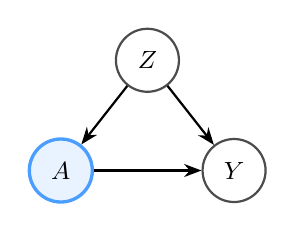
\begin{tikzpicture}
        \node[var]  (Z) at (1.1,1.4) {$Z$};
        \node[tx]   (A) at (0,0)     {$A$};
        \node[outc] (Y) at (2.2,0)   {$Y$};
        \draw[edge] (Z) -- (A);
        \draw[edge] (Z) -- (Y);
        \draw[edge] (A) -- (Y);
      \end{tikzpicture}\\[0.9em]
      \textcolor{good}{\textbf{Adjust for $Z$}} to close the backdoor.
    \end{column}
    \begin{column}{0.52\textwidth}
      \centering
      \textbf{Example: frailty}\\ {\scriptsize sicker patients get the aggressive drug}\\[0.9em]
      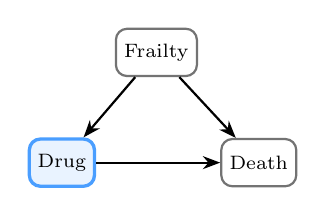
\begin{tikzpicture}
        \node[lab]   (F) at (1.2,1.4) {Frailty};
        \node[labtx] (D) at (0,0)     {Drug};
        \node[lab]   (M) at (2.5,0)   {Death};
        \draw[edge] (F) -- (D);
        \draw[edge] (F) -- (M);
        \draw[edge] (D) -- (M);
      \end{tikzpicture}\\[0.9em]
      {\scriptsize Frailty drives both treatment \emph{and} death, so the crude contrast makes the drug look harmful.}
    \end{column}
  \end{columns}
\end{frame}
% NOTE (Kathryn): The friendly one. Z is a genuine common cause measured
% before treatment; adjusting for it removes the bias. This is the only one
% of the three where "adjust" is the right instinct.

% --- Mediator ---
\begin{frame}{Mediator: On the Causal Path}
  \small
  \begin{columns}[T]
    \begin{column}{0.46\textwidth}
      \centering
      \textbf{Generic structure}\\ {\scriptsize chain: \ $A \to Z \to Y$}\\[0.9em]
      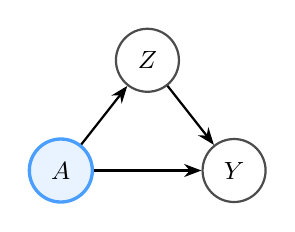
\begin{tikzpicture}
        \node[var]  (Z) at (1.1,1.4) {$Z$};
        \node[tx]   (A) at (0,0)     {$A$};
        \node[outc] (Y) at (2.2,0)   {$Y$};
        \draw[edge] (A) -- (Z);
        \draw[edge] (Z) -- (Y);
        \draw[edge] (A) -- (Y);
      \end{tikzpicture}\\[0.9em]
      \textcolor{brick}{\textbf{Do not adjust}} (for a total effect).
    \end{column}
    \begin{column}{0.52\textwidth}
      \centering
      \textbf{Example: statin and LDL}\\ {\scriptsize the drug acts \emph{through} lowering LDL}\\[0.9em]
      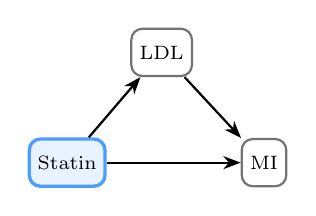
\begin{tikzpicture}
        \node[lab]   (L) at (1.2,1.4) {LDL};
        \node[labtx] (S) at (0,0)     {Statin};
        \node[lab]   (I) at (2.5,0)   {MI};
        \draw[edge] (S) -- (L);
        \draw[edge] (L) -- (I);
        \draw[edge] (S) -- (I);
      \end{tikzpicture}\\[0.9em]
      {\scriptsize Adjust for LDL and the statin looks inert -- you have removed the pathway it acts through.}
    \end{column}
  \end{columns}
\end{frame}
% NOTE (Kathryn): Z sits between A and Y and is measured AFTER time zero.
% Conditioning on it blocks the very effect you want. Preview the time-zero
% tell: post-baseline variables are prime mediator suspects.

% --- Collider ---
\begin{frame}{Collider: A Common Effect}
  \small
  \begin{columns}[T]
    \begin{column}{0.46\textwidth}
      \centering
      \textbf{Generic structure}\\ {\scriptsize collision: \ $A \to Z \leftarrow Y$}\\[0.9em]
      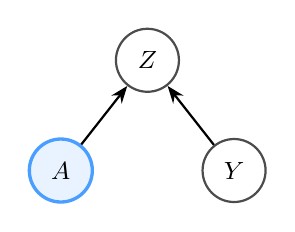
\begin{tikzpicture}
        \node[var]  (Z) at (1.1,1.4) {$Z$};
        \node[tx]   (A) at (0,0)     {$A$};
        \node[outc] (Y) at (2.2,0)   {$Y$};
        \draw[edge] (A) -- (Z);
        \draw[edge] (Y) -- (Z);
      \end{tikzpicture}\\[0.9em]
      \textcolor{brick}{\textbf{Do not adjust}} -- it opens a fake path.
    \end{column}
    \begin{column}{0.52\textwidth}
      \centering
      \textbf{Example: hospitalization}\\ {\scriptsize drug and disease both cause admission}\\[0.9em]
      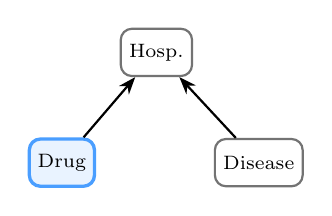
\begin{tikzpicture}
        \node[lab]   (H) at (1.2,1.4) {Hosp.};
        \node[labtx] (D) at (0,0)     {Drug};
        \node[lab]   (X) at (2.5,0)   {Disease};
        \draw[edge] (D) -- (H);
        \draw[edge] (X) -- (H);
      \end{tikzpicture}\\[0.9em]
      {\scriptsize Restrict to the hospitalized and drug and disease look linked. }
    \end{column}
  \end{columns}
\end{frame}
% NOTE (Kathryn): Both arrows point INTO Z. Conditioning on a collider -- by
% adjustment OR by selection/restriction -- creates association not present in
% the population. The Hollywood-actors line lands this fastest.

% ======================================================================
% Slide 6 - Why "adjust for everything" fails
% ======================================================================
\begin{frame}{Why ``Adjust for Everything'' Fails}
  \small
  A single reflex applied to all three does two kinds of damage:
  \vspace{0.6em}

  \begin{columns}[T]
    \begin{column}{0.5\textwidth}
      \textcolor{brick}{\textbf{Adjust a mediator}} \\[0.2em]
      {\footnotesize You block part of the effect you are trying to measure.
      Condition on LDL and the statin looks inert -- you have thrown away
      the mechanism.}
    \end{column}
    \begin{column}{0.5\textwidth}
      \textcolor{brick}{\textbf{Adjust a collider}} \\[0.2em]
      {\footnotesize You \emph{open} a path that was closed. Restrict to
      hospitalized patients and drug and disease look linked when in the
      population they are not.}
    \end{column}
  \end{columns}
  \vspace{1.0em}

  \textcolor{accent}{\textbf{The lesson:}} the covariate list is a set of \emph{claims about structure}, not a bigger-is-safer knob. What to adjust for is decided by the causal question and the diagram, before the data.
  \vspace{0.4em}

  {\footnotesize Which is exactly what Segment D's roadmap makes systematic.}
\end{frame}
% NOTE (Kathryn): This is the conceptual peak. Say plainly: throwing every
% available variable into the model is not caution, it is a modelling choice
% that can manufacture bias. Segue to design.

% ======================================================================
% Slide 7 - Target-trial protocol + time zero
% ======================================================================
\begin{frame}{Design First: The Target Trial}
  \small
  \textbf{Specify the randomized trial you \emph{wish} you could run} \cite{hernan2016target}, then emulate it with the data you have:
  \begin{itemize}
    \item eligibility, treatment strategies, assignment,
    \item follow-up, outcome, and the causal contrast.
  \end{itemize}
  \vspace{0.6em}

  \begin{block}{Time zero: align eligibility, treatment, and follow-up at one instant}
    Every patient's clock starts when they meet eligibility and treatment is
    assigned. Getting this wrong is the classic source of
    \textbf{immortal-time bias} (survival smuggled into the treated group)
    and \textbf{prevalent-user bias} (survivors of early treatment
    overrepresented).
  \end{block}
  \vspace{0.4em}

  \textcolor{accent}{\textbf{Why it matters here:}} a clean time zero is a \emph{design} fix for problems no downstream model can undo.
\end{frame}
% NOTE (Kathryn): This is the bridge to Andy. Time zero is where "design the
% question" stops being a slogan and becomes a concrete rule. Hand the
% protocol structure to Segment D.

% ======================================================================
% Slide 8 - Pneumonia-vaccine paradox
% ======================================================================
\begin{frame}{The Pneumonia-Vaccine Paradox}
  \small
  Observational studies of the pneumococcal vaccine in older adults have
  reported that \textbf{vaccinated patients had \emph{higher} pneumonia risk}
  than the unvaccinated -- the vaccine looks useless, even harmful.
  \vspace{0.5em}

  \textbf{But look at the timing:}
  \begin{itemize}
    \item In a large primary-care cohort, the vaccinated already had higher
      pneumonia rates \emph{in the year before they were vaccinated}.
    \item An ``effect'' that precedes the exposure cannot be caused by it.
    \item The gap is a marker of \emph{who} gets vaccinated, not of harm.
  \end{itemize}
  \vspace{0.5em}

  \begin{block}{Resolution: confounding by indication}
    The vaccine is targeted at frailer, higher-risk patients. Baseline
    frailty is a \textbf{confounder} -- it raises both the chance of
    vaccination \emph{and} the risk of pneumonia. When the trial is actually
    run, the vaccine protects (CAPITA: 46\% against vaccine-type pneumonia)
    \cite{bonten2015capita}.
  \end{block}
\end{frame}
% NOTE (Kathryn): The teachable move is the pre-exposure tell -- the "effect"
% shows up before anyone was vaccinated, so it cannot be the vaccine. Same
% confounder structure as slide 5 (frailty -> treatment and outcome), and the
% SAME direction: sicker patients get treated, so the crude contrast makes the
% treatment look harmful. Contrast with the healthy-vaccinee flu story if the
% room wants it: same fork, opposite sign on the arrow into treatment.

% ======================================================================
% Slide 9 - Handoff
% ======================================================================
\begin{frame}[standout]
  We do not solve this with a better model first.\\[0.8em]
  We solve it by \textbf{designing the question}.
\end{frame}
% NOTE (Kathryn): Beat of silence, then hand to Andy for the roadmap. This
% line is the spine of the whole day; let it sit.

% ======================================================================
% ======================  POLL BANK (backup)  ==========================
% Self-contained. Jump in at any point; skip freely to manage the clock.
% Each poll: options A/B/C on the slide, answer + cue in the NOTE.
% ======================================================================

\begin{frame}[plain]
  \centering
  \vfill
  {\usebeamerfont{title}\color{inkdark}\textbf{\Large Poll Bank}}\\[0.6em]
  {\normalsize Vote in chat: A, B, or C}
  \vfill
\end{frame}
% NOTE (Kathryn): These are flexible fillers. Use the ones that fit the room
% and the clock. Order does not matter. Read the scenario, count votes in
% chat, then reveal.

% --- Poll 1: confounder ---
\begin{frame}{Poll 1 \;--\; Classify the Variable}
  \small
  In a study of a new anticoagulant versus an older one, \textbf{baseline kidney
  function} predicts both which drug the physician prescribes and the risk of
  a bleeding event.
  \vspace{0.8em}

  Baseline kidney function is a:
  \begin{itemize}
    \item[\textbf{A.}] Confounder
    \item[\textbf{B.}] Mediator
    \item[\textbf{C.}] Collider
  \end{itemize}
\end{frame}
% NOTE (Kathryn): Answer A. Measured before treatment, causes both A and Y --
% textbook fork. Adjust for it. Easy warm-up to build voting confidence.

\begin{frame}{Poll 1 \;--\; Solution}
  \small
  \begin{columns}[T]
    \begin{column}{0.52\textwidth}
      \textcolor{good}{\textbf{A -- Confounder.}}\\[0.4em]
      Baseline kidney function is measured \emph{before} treatment and causes
      both the drug choice and bleeding -- a common cause (fork).\\[0.4em]
      \textcolor{accent}{\textbf{Action:}} adjust to close the backdoor.
    \end{column}
    \begin{column}{0.44\textwidth}
      \centering
      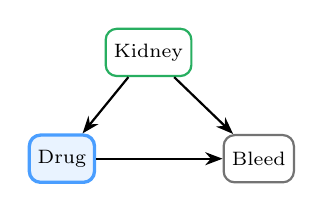
\begin{tikzpicture}
        \node[lab,draw=good] (Z) at (1.1,1.35) {Kidney};
        \node[labtx] (A) at (0,0)   {Drug};
        \node[lab]   (Y) at (2.5,0) {Bleed};
        \draw[edge] (Z) -- (A);
        \draw[edge] (Z) -- (Y);
        \draw[edge] (A) -- (Y);
      \end{tikzpicture}\\[0.3em]
      {\scriptsize\textcolor{good}{green = adjust for it}}
    \end{column}
  \end{columns}
\end{frame}

% --- Poll 2: mediator ---
\begin{frame}{Poll 2 \;--\; Classify the Variable}
  \small
  A blood-pressure drug reduces stroke risk. You have a measurement of
  \textbf{on-treatment blood pressure at 6 months}. You want the
  \emph{total} effect of the drug on stroke.
  \vspace{0.8em}

  On-treatment blood pressure is a:
  \begin{itemize}
    \item[\textbf{A.}] Confounder -- adjust for it
    \item[\textbf{B.}] Mediator -- do not adjust
    \item[\textbf{C.}] Collider -- do not adjust
  \end{itemize}
\end{frame}
% NOTE (Kathryn): Answer B. It sits on the causal path (drug -> BP -> stroke)
% and is measured after time zero. Adjusting for it removes the drug's main
% mechanism. Note the time-zero tell: it is post-baseline.

\begin{frame}{Poll 2 \;--\; Solution}
  \small
  \begin{columns}[T]
    \begin{column}{0.52\textwidth}
      \textcolor{good}{\textbf{B -- Mediator.}}\\[0.4em]
      On-treatment blood pressure lies on the path (drug $\to$ BP $\to$ stroke)
      and is measured \emph{after} time zero.\\[0.4em]
      \textcolor{brick}{\textbf{Do not adjust}} for a total effect.
    \end{column}
    \begin{column}{0.44\textwidth}
      \centering
      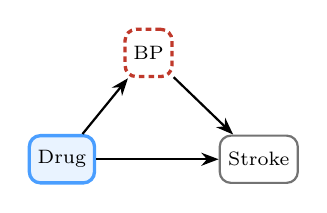
\begin{tikzpicture}
        \node[cond]  (Z) at (1.1,1.35) {BP};
        \node[labtx] (A) at (0,0)   {Drug};
        \node[lab]   (Y) at (2.5,0) {Stroke};
        \draw[edge] (A) -- (Z);
        \draw[edge] (Z) -- (Y);
        \draw[edge] (A) -- (Y);
      \end{tikzpicture}\\[0.3em]
      {\scriptsize\textcolor{brick}{red box = do not condition}}
    \end{column}
  \end{columns}
\end{frame}

% --- Poll 3: collider (the memorable one) ---
\begin{frame}{Poll 3 \;--\; Classify the Variable}
  \small
  Among \textbf{hospitalized} patients only, a drug's side effects and the
  underlying disease both raise the chance of admission. You analyze within
  the hospitalized group.
  \vspace{0.8em}

  Hospitalization (the variable you restricted on) is a:
  \begin{itemize}
    \item[\textbf{A.}] Confounder
    \item[\textbf{B.}] Mediator
    \item[\textbf{C.}] Collider
  \end{itemize}
\end{frame}
% NOTE (Kathryn): Answer C. Both A and disease point INTO admission.
% Restricting to hospitalized conditions on the collider and manufactures a
% drug-disease association. This is selection bias by another name.

\begin{frame}{Poll 3 \;--\; Solution}
  \small
  \begin{columns}[T]
    \begin{column}{0.52\textwidth}
      \textcolor{good}{\textbf{C -- Collider.}}\\[0.4em]
      Side effects and disease both cause admission, so both arrows point
      \emph{into} hospitalization.\\[0.4em]
      \textcolor{brick}{\textbf{Restricting}} to it opens a fake link.
    \end{column}
    \begin{column}{0.44\textwidth}
      \centering
      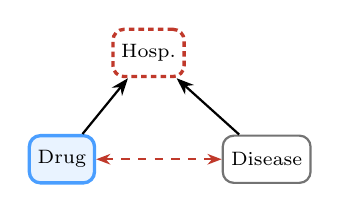
\begin{tikzpicture}
        \node[cond]  (Z) at (1.1,1.35) {Hosp.};
        \node[labtx] (A) at (0,0)   {Drug};
        \node[lab]   (Y) at (2.6,0) {Disease};
        \draw[edge] (A) -- (Z);
        \draw[edge] (Y) -- (Z);
        \draw[spur] (A) -- (Y);
      \end{tikzpicture}\\[0.3em]
      {\scriptsize\textcolor{brick}{dashed = induced association}}
    \end{column}
  \end{columns}
\end{frame}

% --- Poll 4: M-bias trap (deliberately tricky) ---
\begin{frame}{Poll 4 \;--\; The Tricky One}
  \small
  A variable $Z$ is measured \emph{before} treatment. It is caused by two
  unmeasured factors: one that also causes treatment, and one that also
  causes the outcome. $Z$ itself does \emph{not} cause $A$ or $Y$.
  \vspace{0.8em}

  Should you adjust for $Z$?
  \begin{itemize}
    \item[\textbf{A.}] Yes -- it is pre-treatment, so it is safe
    \item[\textbf{B.}] No -- adjusting opens a biasing path
    \item[\textbf{C.}] It never matters either way
  \end{itemize}
\end{frame}
% NOTE (Kathryn): Answer B. This is M-bias. Z is a collider on a path between
% the two unmeasured causes. "Pre-treatment" does NOT equal "safe to adjust."
% Kills the reflex that timing alone licenses adjustment. Use only if the
% room is strong -- it is the hardest poll here.

\begin{frame}{Poll 4 \;--\; Solution}
  \small
  \begin{columns}[T]
    \begin{column}{0.5\textwidth}
      \textcolor{good}{\textbf{B -- do not adjust (M-bias).}}\\[0.4em]
      $Z$ is a collider between two unmeasured causes. Conditioning on it opens
      the $U_1\!\cdots\!U_2$ path and biases $A \to Y$.\\[0.3em]
      \textcolor{brick}{``Pre-treatment'' $\neq$ ``safe.''}
    \end{column}
    \begin{column}{0.46\textwidth}
      \centering
      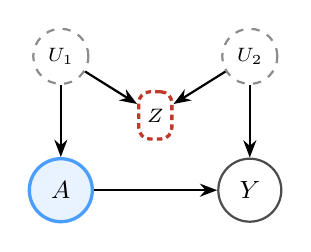
\begin{tikzpicture}
        \node[un]   (U1) at (0,1.7)   {$U_1$};
        \node[un]   (U2) at (2.4,1.7) {$U_2$};
        \node[cond] (Z)  at (1.2,0.95) {$Z$};
        \node[tx]   (A)  at (0,0)   {$A$};
        \node[outc] (Y)  at (2.4,0) {$Y$};
        \draw[edge] (U1) -- (Z);
        \draw[edge] (U2) -- (Z);
        \draw[edge] (U1) -- (A);
        \draw[edge] (U2) -- (Y);
        \draw[edge] (A) -- (Y);
      \end{tikzpicture}\\[0.2em]
      {\scriptsize dashed circle = unmeasured}
    \end{column}
  \end{columns}
\end{frame}

% --- Poll 5: time-zero trap ---
\begin{frame}{Poll 5 \;--\; What Is Wrong With This Comparison?}
  \small
  Patients who filled a prescription for the drug \emph{within the first year}
  are labelled ``treated''; everyone else is ``untreated.'' Survival is
  compared from cohort entry.
  \vspace{0.8em}

  The main problem is:
  \begin{itemize}
    \item[\textbf{A.}] Too small a sample
    \item[\textbf{B.}] Immortal time -- the treated had to survive long enough to fill it
    \item[\textbf{C.}] Measurement error in the outcome
  \end{itemize}
\end{frame}
% NOTE (Kathryn): Answer B. To be classified treated, a patient must survive
% to the fill date -- that survival time is "immortal" and biases toward the
% drug. Fix: align time zero at the moment of treatment assignment. This is
% the direct set-up for Andy's Segment D.

\begin{frame}{Poll 5 \;--\; Solution}
  \small
  \begin{columns}[T]
    \begin{column}{0.5\textwidth}
      \textcolor{good}{\textbf{B -- Immortal time.}}\\[0.4em]
      To be labelled ``treated,'' a patient must survive to the fill date. That
      guaranteed window biases toward the drug.\\[0.3em]
      \textcolor{accent}{\textbf{Fix:}} start time zero at treatment assignment.
    \end{column}
    \begin{column}{0.46\textwidth}
      \centering
      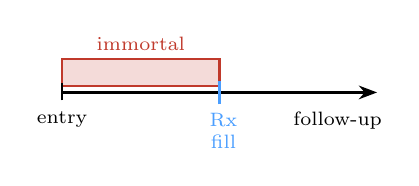
\begin{tikzpicture}[font=\scriptsize]
        \fill[brick!18] (0,0.08) rectangle (2,0.42);
        \draw[brick,thick] (0,0.08) rectangle (2,0.42);
        \node[brick] at (1,0.62) {immortal};
        \draw[thick,-{Stealth}] (0,0) -- (4,0);
        \draw[thick] (0,-0.1) -- (0,0.12); \node[below] at (0,-0.12) {entry};
        \draw[accent,very thick] (2,-0.15) -- (2,0.15);
        \node[accent,below,align=center] at (2.05,-0.14) {Rx\\fill};
        \node[below] at (3.5,-0.12) {follow-up};
      \end{tikzpicture}\\[0.5em]
      {\scriptsize survival in the shaded window is guaranteed}
    \end{column}
  \end{columns}
\end{frame}
% NOTE (Kathryn): a timeline, not a DAG -- immortal time is about where the
% clock starts, which a DAG does not show.

% --- Poll 6: vaccine-paradox style (best run BEFORE slide 8) ---
\begin{frame}{Poll 6 \;--\; Is This Causal?}
  \small
  A study finds that older adults who received the \textbf{pneumonia vaccine}
  have \emph{higher} rates of pneumonia than those who did not.
  \vspace{0.8em}

  The most likely explanation is:
  \begin{itemize}
    \item[\textbf{A.}] The vaccine causes pneumonia
    \item[\textbf{B.}] Sicker, higher-risk patients were the ones vaccinated
    \item[\textbf{C.}] Random chance
  \end{itemize}
\end{frame}
% NOTE (Kathryn): Answer B, confounding by indication. Optionally run this
% BEFORE slide 8 so the reveal IS the content. The clinching tell (save it for
% the discussion): the vaccinated often had higher pneumonia rates even BEFORE
% they were vaccinated, so the gap cannot be an effect of the vaccine.

\begin{frame}{Poll 6 \;--\; Solution}
  \small
  \begin{columns}[T]
    \begin{column}{0.52\textwidth}
      \textcolor{good}{\textbf{B -- confounding by indication.}}\\[0.4em]
      Frailer patients are targeted for the vaccine, so frailty raises both
      vaccination and pneumonia risk.\\[0.4em]
      \textcolor{accent}{\textbf{Tell:}} the gap predates vaccination.
    \end{column}
    \begin{column}{0.44\textwidth}
      \centering
      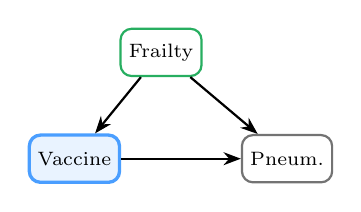
\begin{tikzpicture}
        \node[lab,draw=good] (Z) at (1.1,1.35) {Frailty};
        \node[labtx] (A) at (0,0)   {Vaccine};
        \node[lab]   (Y) at (2.7,0) {Pneum.};
        \draw[edge] (Z) -- (A);
        \draw[edge] (Z) -- (Y);
        \draw[edge] (A) -- (Y);
      \end{tikzpicture}\\[0.3em]
      {\scriptsize frailty confounds the crude contrast}
    \end{column}
  \end{columns}
\end{frame}

% --- Poll 7: confounder vs mediator by timing ---
\begin{frame}{Poll 7 \;--\; Which Is Safe to Adjust For?}
  \small
  In a statin study you could adjust for LDL cholesterol measured \emph{at
  baseline}, or LDL measured \emph{at 6 months on treatment}. You want the
  \textbf{total} effect of the statin on heart attacks.
  \vspace{0.8em}

  Which is safe to adjust for?
  \begin{itemize}
    \item[\textbf{A.}] Baseline LDL
    \item[\textbf{B.}] On-treatment LDL
    \item[\textbf{C.}] Both, to be safe
  \end{itemize}
\end{frame}
% NOTE (Kathryn): Answer A. Baseline LDL is a pre-treatment confounder;
% on-treatment LDL is a mediator and blocks the drug's pathway. "Both" is the
% trap that catches the adjust-for-everything reflex. Reinforces time zero.

\begin{frame}{Poll 7 \;--\; Solution}
  \small
  \begin{columns}[T]
    \begin{column}{0.48\textwidth}
      \textcolor{good}{\textbf{A -- baseline LDL only.}}\\[0.4em]
      \textcolor{good}{Baseline LDL} is a pre-treatment confounder (adjust).
      \textcolor{brick}{On-treatment LDL} is a mediator (do not).\\[0.3em]
      Same variable, two roles -- set by timing.
    \end{column}
    \begin{column}{0.48\textwidth}
      \centering
      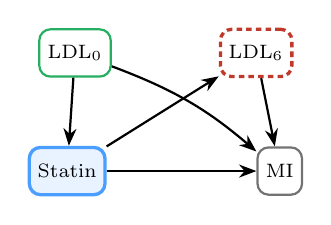
\begin{tikzpicture}[font=\scriptsize]
        \node[lab,draw=good] (L0) at (0.1,1.5) {LDL$_0$};
        \node[cond]          (L6) at (2.4,1.5) {LDL$_6$};
        \node[labtx] (A) at (0,0)   {Statin};
        \node[lab]   (Y) at (2.7,0) {MI};
        \draw[edge] (L0) -- (A);
        \draw[edge] (L0) to[bend left=10] (Y);
        \draw[edge] (A) -- (L6);
        \draw[edge] (L6) -- (Y);
        \draw[edge] (A) -- (Y);
      \end{tikzpicture}\\[0.2em]
      {\scriptsize\textcolor{good}{green=adjust}\ \ \textcolor{brick}{red=don't}}
    \end{column}
  \end{columns}
\end{frame}

% --- Poll 8: Simpson's paradox ---
\begin{frame}{Poll 8 \;--\; Simpson's Paradox}
  \small
  Pooled together, patients on the new drug have \emph{higher} mortality than
  those on the old drug. But within \emph{every} disease-severity stratum, the
  new drug has \emph{lower} mortality.
  \vspace{0.8em}

  Which comparison reflects the drug's effect?
  \begin{itemize}
    \item[\textbf{A.}] The pooled comparison
    \item[\textbf{B.}] The within-severity comparison
    \item[\textbf{C.}] Neither can be trusted
  \end{itemize}
\end{frame}
% NOTE (Kathryn): Answer B -- BUT only because severity is a pre-treatment
% confounder (sicker patients got the new drug). The deeper point: the
% direction to trust depends on WHY you are stratifying. If the stratifier
% were a mediator or collider, stratifying would be the wrong move. Structure,
% not arithmetic, decides.

\begin{frame}{Poll 8 \;--\; Solution}
  \small
  \begin{columns}[T]
    \begin{column}{0.52\textwidth}
      \textcolor{good}{\textbf{B -- within-severity,}} \emph{here}.\\[0.4em]
      Severity is a pre-treatment confounder: sicker patients got the new drug.
      Stratifying removes the bias.\\[0.3em]
      \textcolor{brick}{\textbf{Catch:}} only because the stratifier is a confounder.
    \end{column}
    \begin{column}{0.44\textwidth}
      \centering
      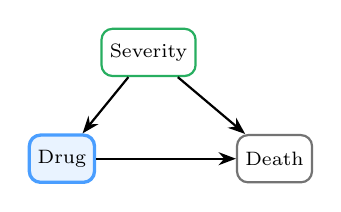
\begin{tikzpicture}
        \node[lab,draw=good] (Z) at (1.1,1.35) {Severity};
        \node[labtx] (A) at (0,0)   {Drug};
        \node[lab]   (Y) at (2.7,0) {Death};
        \draw[edge] (Z) -- (A);
        \draw[edge] (Z) -- (Y);
        \draw[edge] (A) -- (Y);
      \end{tikzpicture}\\[0.3em]
      {\scriptsize stratify on a confounder, not a mediator}
    \end{column}
  \end{columns}
\end{frame}

% --- Poll 9: healthy adherer bias ---
\begin{frame}{Poll 9 \;--\; The Adherent Placebo Patient}
  \small
  In a randomized trial, patients who took their \textbf{placebo} as prescribed
  had substantially \emph{lower} mortality than patients who did not adhere to
  the placebo.
  \vspace{0.8em}

  The best explanation is:
  \begin{itemize}
    \item[\textbf{A.}] The placebo had a real effect
    \item[\textbf{B.}] Adherence is a marker of healthier behaviour overall
    \item[\textbf{C.}] The randomization failed
  \end{itemize}
\end{frame}
% NOTE (Kathryn): Answer B, the healthy-adherer effect (Coronary Drug
% Project). Adherence tracks health-seeking behaviour and baseline health, not
% a pill effect. This is why per-protocol and adherence analyses can smuggle
% confounding into a randomized trial. A favourite "clean but biased" case.

\begin{frame}{Poll 9 \;--\; Solution}
  \small
  \begin{columns}[T]
    \begin{column}{0.52\textwidth}
      \textcolor{good}{\textbf{B -- healthy-adherer bias.}}\\[0.4em]
      Adhering even to placebo marks healthier, more health-conscious people.
      Adherence is a confounded proxy, not a cause.\\[0.3em]
      Randomization protects the \emph{assigned} contrast only.
    \end{column}
    \begin{column}{0.44\textwidth}
      \centering
      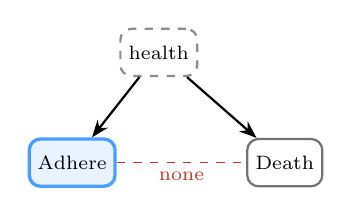
\begin{tikzpicture}
        \node[lab,dashed,draw=black!45] (U) at (1.1,1.4) {health};
        \node[labtx] (A) at (0,0)   {Adhere};
        \node[lab]   (Y) at (2.7,0) {Death};
        \draw[edge] (U) -- (A);
        \draw[edge] (U) -- (Y);
        \draw[dashed,brick] (A) -- (Y) node[midway,below,font=\scriptsize,brick]{none};
      \end{tikzpicture}\\[0.3em]
      {\scriptsize unmeasured health drives both}
    \end{column}
  \end{columns}
\end{frame}

% --- Poll 10: protopathic bias / reverse causation ---
\begin{frame}{Poll 10 \;--\; The Painkiller and the Cancer}
  \small
  A painkiller is prescribed for early back pain. Months later, some of those
  patients are diagnosed with spinal cancer -- which had been causing the pain
  all along. In the data, the painkiller is associated with cancer.
  \vspace{0.8em}

  This is:
  \begin{itemize}
    \item[\textbf{A.}] A real carcinogenic effect
    \item[\textbf{B.}] Reverse causation: early symptoms of the outcome triggered the drug
    \item[\textbf{C.}] Confounding by age
  \end{itemize}
\end{frame}
% NOTE (Kathryn): Answer B, protopathic bias. The outcome (its early symptoms)
% caused the treatment, not the other way round. Fix: a lag / exclusion window
% between time zero and outcome ascertainment so early disease cannot drive the
% exposure. Very RWE-relevant.

\begin{frame}{Poll 10 \;--\; Solution}
  \small
  \begin{columns}[T]
    \begin{column}{0.52\textwidth}
      \textcolor{good}{\textbf{B -- reverse causation.}}\\[0.4em]
      Undiagnosed cancer caused the pain that led to the drug. The arrow runs
      outcome $\to$ exposure.\\[0.3em]
      \textcolor{accent}{\textbf{Fix:}} a lag/exclusion window before time zero.
    \end{column}
    \begin{column}{0.44\textwidth}
      \centering
      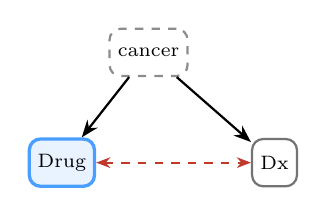
\begin{tikzpicture}
        \node[lab,dashed,draw=black!45] (C) at (1.1,1.4) {cancer};
        \node[labtx] (A) at (0,0)   {Drug};
        \node[lab]   (Y) at (2.7,0) {Dx};
        \draw[edge] (C) -- (A);
        \draw[edge] (C) -- (Y);
        \draw[spur] (A) -- (Y);
      \end{tikzpicture}\\[0.3em]
      {\scriptsize the ``effect'' is driven by latent disease}
    \end{column}
  \end{columns}
\end{frame}

% --- Poll 11: Table 2 fallacy ---
\begin{frame}{Poll 11 \;--\; The Table 2 Fallacy}
  \small
  A model estimates a drug's effect on stroke, adjusting for age, smoking, and
  hypertension. The results table also reports the \textbf{smoking} coefficient
  and the paper reads it as ``the effect of smoking on stroke.''
  \vspace{0.8em}

  Is that smoking coefficient a valid causal effect of smoking?
  \begin{itemize}
    \item[\textbf{A.}] Yes -- it was adjusted for the same covariates
    \item[\textbf{B.}] Not generally -- the adjustment set was chosen for the drug, not for smoking
    \item[\textbf{C.}] Yes, always
  \end{itemize}
\end{frame}
% NOTE (Kathryn): Answer B, the Table 2 fallacy. An adjustment set that
% identifies the drug effect will not, in general, identify each covariate's
% own effect: some covariates are confounded, others may be mediators of
% smoking. One model, one estimand. HEOR audiences see this constantly.

\begin{frame}{Poll 11 \;--\; Solution}
  \small
  \begin{columns}[T]
    \begin{column}{0.5\textwidth}
      \textcolor{good}{\textbf{B -- not generally valid.}}\\[0.4em]
      The set that identifies the \emph{drug} effect need not identify
      smoking's: adjusting HTN (a mediator of smoking) blocks part of its own
      effect.\\[0.2em]
      One model, one estimand.
    \end{column}
    \begin{column}{0.46\textwidth}
      \centering
      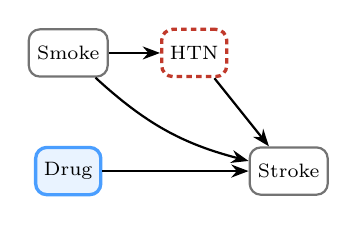
\begin{tikzpicture}[font=\scriptsize]
        \node[lab]  (S) at (0,1.5)   {Smoke};
        \node[cond] (H) at (1.6,1.5) {HTN};
        \node[labtx] (D) at (0,0)    {Drug};
        \node[lab]   (Y) at (2.8,0)  {Stroke};
        \draw[edge] (S) -- (H);
        \draw[edge] (H) -- (Y);
        \draw[edge] (S) to[bend right=14] (Y);
        \draw[edge] (D) -- (Y);
      \end{tikzpicture}\\[0.2em]
      {\scriptsize adjusting HTN: right for Drug, wrong for Smoke}
    \end{column}
  \end{columns}
\end{frame}

% --- Poll 12: time-varying confounding ---
\begin{frame}{Poll 12 \;--\; The Feedback Loop}
  \small
  In an HIV study, CD4 count is \emph{affected by} prior antiretroviral
  treatment, \emph{predicts} whether treatment continues, and \emph{predicts}
  mortality. You want the effect of sustained treatment on mortality.
  \vspace{0.8em}

  Standard regression adjusting for CD4:
  \begin{itemize}
    \item[\textbf{A.}] Works fine -- CD4 is a confounder, so adjust for it
    \item[\textbf{B.}] Is biased -- CD4 both confounds later treatment \emph{and} is affected by earlier treatment
    \item[\textbf{C.}] Should ignore CD4 entirely
  \end{itemize}
\end{frame}
% NOTE (Kathryn): Answer B, time-varying confounding. CD4 is a confounder of
% later treatment that is itself on the pathway from earlier treatment.
% Adjusting for it blocks part of the effect AND opens collider bias; omitting
% it leaves confounding. Neither plain option works -- you need g-methods
% (g-computation, IPW, TMLE). Direct hook into Andy's Segment G.

\begin{frame}{Poll 12 \;--\; Solution}
  \small
  \begin{columns}[T]
    \begin{column}{0.48\textwidth}
      \textcolor{good}{\textbf{B -- time-varying confounder.}}\\[0.4em]
      CD4 is affected by early treatment \emph{and} confounds later treatment.
      Adjust and you block/collide; omit and you confound.\\[0.2em]
      \textcolor{accent}{\textbf{Use g-methods.}}
    \end{column}
    \begin{column}{0.48\textwidth}
      \centering
      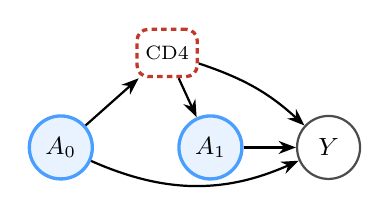
\begin{tikzpicture}[font=\scriptsize]
        \node[tx]   (A0) at (0,0)    {$A_0$};
        \node[cond] (L)  at (1.35,1.2) {CD4};
        \node[tx]   (A1) at (1.9,0)  {$A_1$};
        \node[outc] (Y)  at (3.4,0)  {$Y$};
        \draw[edge] (A0) -- (L);
        \draw[edge] (L) -- (A1);
        \draw[edge] (A1) -- (Y);
        \draw[edge] (L) to[bend left=12] (Y);
        \draw[edge] (A0) to[bend right=24] (Y);
      \end{tikzpicture}\\[0.2em]
      {\scriptsize CD4: mediator of $A_0$, confounder of $A_1$}
    \end{column}
  \end{columns}
\end{frame}

% --- Poll 13: instrument ---
\begin{frame}{Poll 13 \;--\; Spot the Instrument}
  \small
  You want an \textbf{instrument} for whether a patient receives the new drug.
  Which candidate is the most plausible?
  \vspace{0.8em}

  \begin{itemize}
    \item[\textbf{A.}] Baseline disease severity
    \item[\textbf{B.}] The prescribing physician's general preference for the new drug
    \item[\textbf{C.}] The patient's on-treatment lab values
  \end{itemize}
\end{frame}
% NOTE (Kathryn): Answer B. A valid instrument affects treatment but influences
% the outcome ONLY through treatment. Physician preference fits (subject to
% strong, largely untestable assumptions). A is a confounder (affects outcome
% directly); C is a mediator (post-treatment). Good bridge to IV methods.

\begin{frame}{Poll 13 \;--\; Solution}
  \small
  \begin{columns}[T]
    \begin{column}{0.5\textwidth}
      \textcolor{good}{\textbf{B -- physician preference.}}\\[0.4em]
      An instrument moves treatment but reaches $Y$ \emph{only through} it.
      Severity is a confounder; labs are a mediator.\\[0.2em]
      \textcolor{brick}{Assumptions are strong, untestable.}
    \end{column}
    \begin{column}{0.46\textwidth}
      \centering
      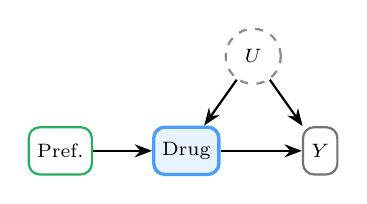
\begin{tikzpicture}[font=\scriptsize]
        \node[lab,draw=good] (Z) at (0,0)   {Pref.};
        \node[labtx] (A) at (1.6,0) {Drug};
        \node[lab]   (Y) at (3.3,0) {$Y$};
        \node[un]    (U) at (2.45,1.2) {$U$};
        \draw[edge] (Z) -- (A);
        \draw[edge] (A) -- (Y);
        \draw[edge] (U) -- (A);
        \draw[edge] (U) -- (Y);
      \end{tikzpicture}\\[0.2em]
      {\scriptsize instrument sidesteps unmeasured $U$}
    \end{column}
  \end{columns}
\end{frame}

% --- Poll 14: positivity ---
\begin{frame}{Poll 14 \;--\; No Comparison Group}
  \small
  Clinical guidelines mandate the drug for \emph{everyone} with severe disease,
  so in your data there are \textbf{zero untreated} severe patients.
  \vspace{0.8em}

  For the severe subgroup, you:
  \begin{itemize}
    \item[\textbf{A.}] Can still estimate the effect by adjusting
    \item[\textbf{B.}] Cannot estimate it -- there is no comparison group
    \item[\textbf{C.}] Should impute the missing untreated patients
  \end{itemize}
\end{frame}
% NOTE (Kathryn): Answer B, a positivity (overlap) violation. With no untreated
% severe patients, the effect in that stratum is not identified -- no model
% fixes it, and "imputing" the counterfactual group is extrapolation, not
% inference. This is a roadmap identification check, previews Segment D.

\begin{frame}{Poll 14 \;--\; Solution}
  \small
  \begin{columns}[T]
    \begin{column}{0.5\textwidth}
      \textcolor{good}{\textbf{B -- positivity violation.}}\\[0.4em]
      Identification needs both arms within each stratum. With no untreated
      severe patients, that effect is not in the data.\\[0.2em]
      \textcolor{brick}{Imputing the arm is extrapolation.}
    \end{column}
    \begin{column}{0.46\textwidth}
      \centering
      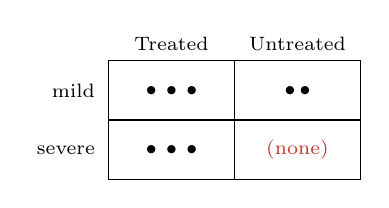
\begin{tikzpicture}[font=\scriptsize]
        \draw (0,0) rectangle (3.2,1.5);
        \draw (1.6,0) -- (1.6,1.5);
        \draw (0,0.75) -- (3.2,0.75);
        \node at (0.8,1.72) {Treated}; \node at (2.4,1.72) {Untreated};
        \node[left] at (-0.05,1.12) {mild}; \node[left] at (-0.05,0.37) {severe};
        \node at (0.8,1.12) {$\bullet\,\bullet\,\bullet$};
        \node at (2.4,1.12) {$\bullet\,\bullet$};
        \node at (0.8,0.37) {$\bullet\,\bullet\,\bullet$};
        \node[brick] at (2.4,0.37) {(none)};
      \end{tikzpicture}\\[0.3em]
      {\scriptsize no untreated severe patients = no contrast}
    \end{column}
  \end{columns}
\end{frame}
% NOTE (Kathryn): an overlap schematic, not a DAG -- positivity is about data
% support, which a DAG does not capture.

% --- Poll 15: differential dropout ---
\begin{frame}{Poll 15 \;--\; The Completers Analysis}
  \small
  In a cohort, treated patients who do poorly tend to drop out early, while
  untreated patients who do poorly stay in. You analyze only the patients who
  \textbf{completed} follow-up.
  \vspace{0.8em}

  Restricting to completers:
  \begin{itemize}
    \item[\textbf{A.}] Is fine -- completers have the cleanest data
    \item[\textbf{B.}] Induces selection bias -- completion is a collider
    \item[\textbf{C.}] Only reduces power
  \end{itemize}
\end{frame}
% NOTE (Kathryn): Answer B. Completion is a common effect of treatment and
% prognosis, so both arrows point into it. Restricting to completers conditions
% on that collider and manufactures a treatment-outcome association. Same
% machinery as Poll 3, wearing the costume of "sensible data cleaning."

\begin{frame}{Poll 15 \;--\; Solution}
  \small
  \begin{columns}[T]
    \begin{column}{0.52\textwidth}
      \textcolor{good}{\textbf{B -- collider selection bias.}}\\[0.4em]
      Completing follow-up is a common effect of treatment and prognosis.
      Keeping only completers conditions on that collider.\\[0.3em]
      \textcolor{brick}{Same structure as Poll 3.}
    \end{column}
    \begin{column}{0.44\textwidth}
      \centering
      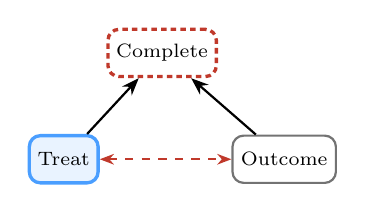
\begin{tikzpicture}
        \node[cond]  (Z) at (1.25,1.35) {Complete};
        \node[labtx] (A) at (0,0)   {Treat};
        \node[lab]   (Y) at (2.8,0) {Outcome};
        \draw[edge] (A) -- (Z);
        \draw[edge] (Y) -- (Z);
        \draw[spur] (A) -- (Y);
      \end{tikzpicture}\\[0.3em]
      {\scriptsize conditioning on completion opens a path}
    \end{column}
  \end{columns}
\end{frame}

% --- Poll 16: lead-time bias ---
\begin{frame}{Poll 16 \;--\; Screening ``Adds a Year''}
  \small
  Patients whose cancer is found by \textbf{screening} survive on average 3
  years from diagnosis; those found after \textbf{symptoms} survive 2 years.
  Screening appears to add a year of life.
  \vspace{0.8em}

  The most likely explanation is:
  \begin{itemize}
    \item[\textbf{A.}] Screening genuinely extends life by a year
    \item[\textbf{B.}] Lead-time bias -- earlier diagnosis just starts the clock sooner
    \item[\textbf{C.}] The screened cancers were less aggressive
  \end{itemize}
\end{frame}
% NOTE (Kathryn): Answer B, lead-time bias. Moving the diagnosis date earlier
% lengthens measured survival-from-diagnosis without postponing death. Option C
% (length-time bias) is a real, related screening artefact worth a mention, but
% B is the one the numbers here describe. Good "time zero for the outcome
% clock" companion to the immortal-time poll.

\begin{frame}{Poll 16 \;--\; Solution}
  \small
  \begin{columns}[T]
    \begin{column}{0.5\textwidth}
      \textcolor{good}{\textbf{B -- lead-time bias.}}\\[0.4em]
      Screening moves the diagnosis date earlier. Survival \emph{from
      diagnosis} stretches even if death never moves.\\[0.3em]
      An artefact of where the clock starts.
    \end{column}
    \begin{column}{0.46\textwidth}
      \centering
      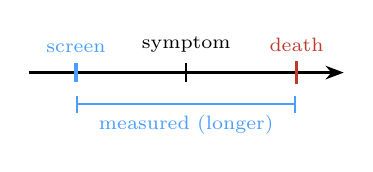
\begin{tikzpicture}[font=\scriptsize]
        \draw[thick,-{Stealth}] (0,0) -- (4,0);
        \draw[accent,very thick] (0.6,-0.12) -- (0.6,0.12);
        \node[accent,above] at (0.6,0.13) {screen};
        \draw[thick] (2,-0.12) -- (2,0.12); \node[above] at (2,0.13) {symptom};
        \draw[brick,very thick] (3.4,-0.15) -- (3.4,0.15);
        \node[brick,above] at (3.4,0.15) {death};
        \draw[accent,thick,{|}-{|}] (0.6,-0.4) -- (3.4,-0.4);
        \node[accent,below] at (2,-0.42) {measured (longer)};
      \end{tikzpicture}\\[0.5em]
      {\scriptsize earlier start, same death date}
    \end{column}
  \end{columns}
\end{frame}
% NOTE (Kathryn): a timeline, not a DAG -- lead-time bias is a clock-start
% artefact. Length-time bias (option C) is a related real screening effect.

% ======================================================================
% Bibliography
% ======================================================================
\begin{frame}[allowframebreaks]{References}
  \tiny
  \bibliographystyle{plainnat}
  \begin{thebibliography}{9}
    \bibitem{hernan2016target}
    Hern{\'a}n MA, Robins JM.
    \newblock Using big data to emulate a target trial when a randomized trial is not available.
    \newblock \textit{American Journal of Epidemiology}, 183(8):758--764, 2016.

    \bibitem{hernan2020causal}
    Hern{\'a}n MA, Robins JM.
    \newblock \textit{Causal Inference: What If}.
    \newblock Chapman \& Hall/CRC, 2020.

    \bibitem{pearl2018why}
    Pearl J, Mackenzie D.
    \newblock \textit{The Book of Why: The New Science of Cause and Effect}.
    \newblock Basic Books, 2018.

    \bibitem{bonten2015capita}
    Bonten MJM, Huijts SM, Bolkenbaas M, et al.
    \newblock Polysaccharide conjugate vaccine against pneumococcal pneumonia in adults.
    \newblock \textit{New England Journal of Medicine}, 372(12):1114--1125, 2015.
  \end{thebibliography}
\end{frame}

\end{document}
